\documentclass[12pt]{article}

\usepackage{sbc-template}
\usepackage{graphicx,url}
\usepackage[T1]{fontenc}
\usepackage[utf8]{inputenc}
\usepackage[brazil]{babel}
\usepackage{amsmath}
\usepackage{array}
\usepackage{float}
\usepackage{placeins}
\usepackage{tikz}
\usetikzlibrary{arrows.meta,positioning,shapes.geometric}

\sloppy

\newcommand{\oracle}{\mbox{\textit{Oracle@3}}}

\title{Chain-of-Thought, Flow of Reasoning e Multi-Trajetória no Gemma 4: um Estudo Experimental de Estratégias de Prompting em SLM Local via LLM-Juiz}

\author{Marcos Hideki Nishida Sakaguchi\inst{1}}

\address{Departamento de Ciências da Computação e Estatística\\
Universidade Estadual Paulista (UNESP)\\
Faculdade de Ciências -- Bauru, SP -- Brasil\\
\email{marcos.sakaguchi@unesp.br}
}

\begin{document}

\maketitle

\begin{abstract}
This paper presents an experimental study comparing prompting strategies in a local Small Language Model executed through Ollama. The study evaluates direct answering, Chain-of-Thought, Flow of Reasoning, and a three-trajectory strategy inspired by GFlowNets over GSM8K, ARC-Challenge, Hendrycks MATH/AIME, and TruthfulQA. Answers are standardized with \texttt{RESPOSTA\_FINAL}, stored in auditable JSON/JSONL files, and assessed through deterministic matching, symbolic equivalence, and an external reference-based LLM-as-a-Judge. In the final round, direct answering reached the highest aggregate accuracy among Gemma 4 conditions (85.4\%), while the structured strategies ranged from 82.5\% to 83.3\%. The results do not support an aggregate gain from structured reasoning under the tested configuration, although \oracle{} indicates unused potential in the multi-trajectory selection step. Nemotron Diffusion is reported separately as an external-model baseline over the same frozen questions.
\end{abstract}

\begin{resumo}
Este trabalho apresenta um estudo experimental para comparar estratégias de prompting em um Small Language Model local executado via Ollama. O estudo avalia resposta direta, Chain-of-Thought, Flow of Reasoning e uma estratégia multi-trajetória inspirada em GFlowNets nos datasets GSM8K, ARC-Challenge, Hendrycks MATH/AIME e TruthfulQA. As respostas são padronizadas com \texttt{RESPOSTA\_FINAL}, armazenadas em JSON/JSONL auditável e avaliadas por comparação determinística, equivalência simbólica e LLM-juiz externo baseado em referência. Na rodada final, a resposta direta obteve a maior acurácia agregada entre as condições do Gemma 4 (85,4\%), enquanto as estratégias estruturadas variaram entre 82,5\% e 83,3\%. Os resultados não sustentam ganho agregado do raciocínio estruturado sob a configuração testada, embora o \oracle{} indique potencial não aproveitado na etapa de seleção multi-trajetória. O Nemotron Diffusion é reportado separadamente como baseline externo de modelo sobre as mesmas perguntas congeladas.
\end{resumo}

\section{Introdução}

Modelos de linguagem de grande porte consolidaram-se como ferramentas de alto desempenho em geração textual, programação, resolução de problemas e análise semântica. Ainda assim, a adoção desses modelos em contextos educacionais, acadêmicos e institucionais frequentemente esbarra em fatores práticos: custo por requisição, latência de rede, dependência de provedores externos, restrições de privacidade e dificuldade de reprodução exata do ambiente. Em oposição a esse cenário, modelos de linguagem pequenos (SLMs) oferecem uma alternativa operacionalmente interessante, pois podem ser executados localmente, permitem maior controle sobre dados e tornam experimentos mais acessíveis em máquinas de consumo.

Essa vantagem operacional, entretanto, não elimina limitações de qualidade. Em modelos menores, erros de raciocínio tendem a aparecer com maior frequência quando a tarefa exige manter várias informações simultaneamente, decompor um enunciado, executar operações aritméticas, verificar hipóteses ou rejeitar premissas falsas. Assim, uma pergunta central para o uso prático de SLMs não é apenas se eles conseguem gerar texto fluente, mas se estratégias de inferência podem melhorar a confiabilidade das respostas sem alterar os pesos do modelo.

Este trabalho investiga essa questão por meio da comparação de técnicas de raciocínio em tempo de inferência. O termo ``tempo de inferência'' é usado para destacar que as intervenções ocorrem no momento em que o modelo responde: alteram-se prompts, formato de resposta, número de trajetórias e etapa de julgamento externo, mas não se realiza fine-tuning. Essa distinção é importante porque técnicas em tempo de inferência são mais simples de aplicar, reversíveis, baratas e compatíveis com diferentes modelos locais.

A proposta compara quatro famílias de abordagem: resposta direta, Chain-of-Thought (CoT), Flow of Reasoning (FoR) e uma estratégia multi-trajetória inspirada em GFlowNets. A resposta direta funciona como linha de base. CoT introduz passos intermediários. FoR organiza esses passos em fases fixas. A abordagem inspirada em GFlowNets gera três trajetórias alternativas e seleciona uma resposta por consenso determinístico, sem acesso ao gabarito. Um modelo avaliador separado e preferencialmente mais forte julga posteriormente todas as estratégias. Essa separação evita que o juiz transforme as três candidatas de \texttt{gflow} em uma vantagem oracular.

O modelo alvo principal é o \texttt{gemma4:e4b}, executado localmente via Ollama. O protocolo, contudo, foi implementado de modo a permitir a troca do modelo por variável de ambiente, o que torna possível repetir o experimento com outros SLMs. O estudo utiliza datasets variados para evitar uma avaliação estreita: GSM8K representa raciocínio aritmético em linguagem natural, ARC-Challenge representa inferência científica de múltipla escolha, Hendrycks MATH/AIME representa matemática de maior complexidade e TruthfulQA representa veracidade e resistência a mitos ou premissas enganosas.

As perguntas de pesquisa que orientam o trabalho são:

\begin{itemize}
\item \textbf{QP1}: estratégias de raciocínio estruturado melhoram a correção das respostas de um SLM local em comparação com resposta direta?
\item \textbf{QP2}: a estratégia multi-trajetória inspirada em GFlowNets oferece ganho suficiente para justificar o aumento de chamadas ao modelo em relação às estratégias de uma única chamada?
\item \textbf{QP3}: o efeito das estratégias muda conforme o tipo de dataset, por exemplo matemática, ciência escolar ou veracidade factual?
\item \textbf{QP4}: a padronização da resposta final e a avaliação por LLM-juiz tornam o processo mais auditável e menos dependente de inspeção manual?
\end{itemize}

As contribuições do trabalho podem ser resumidas em cinco pontos. Primeiro, apresenta-se um protocolo experimental reprodutível para comparar estratégias de inferência em SLMs locais. Segundo, formaliza-se uma adaptação multi-trajetória com seleção por consenso sem gabarito e cálculo separado de \oracle{}. Terceiro, implementa-se um LLM-as-a-Judge externo com auditoria por ordem reversa e suporte a um segundo juiz. Quarto, combinam-se métricas determinísticas, equivalência simbólica, Truthfulness e Informativeness. Quinto, organizam-se scripts para geração, avaliação humana cega, consolidação estatística com bootstrap e visualização gráfica.

O fluxo experimental selecionou 100 instâncias por dataset, executou o modelo sob cada estratégia, padronizou a saída no marcador \texttt{RESPOSTA\_FINAL}, persistiu arquivos JSON/JSONL, combinou avaliação determinística e LLM como juiz, consolidou métricas e gerou gráficos. A rodada final, identificada como \texttt{rodada\_20260624\_040601}, foi concluída com 400 perguntas congeladas, 2000 respostas oficiais quando se soma Gemma e Nemotron, 2000 avaliações determinísticas e 660 avaliações por LLM-juiz. Este artigo descreve os fundamentos conceituais, a metodologia, o desenvolvimento do pipeline e os resultados quantitativos consolidados dessa rodada.


\section{Trabalhos Relacionados}

A fundamentação deste trabalho cruza quatro linhas de pesquisa: estratégias de prompting para raciocínio, avaliação comparativa de SLMs, inferência multi-trajetória e avaliação automatizada por LLM-juiz. Essa organização é importante porque o objetivo do experimento não é apenas medir se um modelo local responde corretamente, mas verificar se diferentes formas de conduzir o mesmo SLM alteram acurácia, custo e robustez em tarefas de natureza distinta.

\subsection{Prompting para Raciocínio Passo a Passo}

O Chain-of-Thought prompting foi proposto por Wei et al. \cite{wei2022} como uma forma de induzir modelos de linguagem a produzir etapas intermediárias antes da resposta final. A intuição é que, ao explicitar uma cadeia textual de raciocínio, o modelo cria um espaço de trabalho no próprio contexto, o que pode beneficiar tarefas aritméticas, simbólicas e de múltiplas etapas. Em vez de responder diretamente, o modelo passa a decompor o enunciado, identificar variáveis relevantes e concluir com uma resposta final.

Kojima et al. \cite{kojima2022} mostram que esse comportamento também pode ser induzido em configuração \textit{zero-shot}, sem exemplos demonstrativos, por meio de instruções simples como ``Let's think step by step''. Essa linha é relevante para o presente artigo porque todas as estratégias testadas são baseadas em prompting, sem fine-tuning ou alteração dos pesos do modelo. Assim, a comparação entre \texttt{base} e \texttt{cot} mede o efeito prático de uma instrução de raciocínio explícito em um SLM local, mantendo constantes modelo, amostra e infraestrutura.

Variações posteriores exploram decomposição e planejamento. Least-to-Most Prompting \cite{zhou2023} transforma problemas complexos em subproblemas sequenciais, enquanto Plan-and-Solve Prompting \cite{wang2023plansolve} separa a etapa de planejamento da etapa de execução para reduzir erros de passos ausentes em Zero-shot-CoT. Essas propostas motivam a estratégia \texttt{for} deste trabalho, que organiza a resposta em decomposição, mapeamento de conhecimento, execução e auditoria. A diferença é que, aqui, essas estruturas são avaliadas comparativamente no mesmo SLM e nos mesmos datasets, em vez de serem tratadas como melhorias presumidas.

\subsection{Benchmarks Comparativos de SLMs}

A literatura recente também passou a avaliar SLMs como uma categoria própria, em vez de analisá-los apenas como versões menores de LLMs. ThinkSLM \cite{thinkslm2025} avalia dezenas de SLMs em múltiplos benchmarks de raciocínio e discute formas de julgamento, incluindo avaliação baseada em regras, avaliação humana e LLM-as-a-Judge. Esse tipo de estudo mostra que a capacidade de raciocínio em modelos pequenos é heterogênea e depende de família de modelo, forma de treinamento, compressão e tipo de tarefa.

SLM-Bench \cite{slmbench2025} amplia essa perspectiva ao comparar diferentes SLMs em tarefas de NLP, datasets variados e configurações de hardware, incorporando métricas de desempenho, computação e consumo. Essa ênfase em eficiência é particularmente relevante para execução local: um modelo ou estratégia não deve ser avaliado apenas pela acurácia, mas também pelo custo de inferência, latência e viabilidade operacional.

O presente trabalho é complementar a esses benchmarks. Enquanto ThinkSLM e SLM-Bench buscam responder quais SLMs apresentam melhor desempenho em conjuntos amplos de tarefas, este artigo fixa um único SLM local e pergunta qual estratégia de prompting compensa dentro desse mesmo modelo. Essa distinção reduz variáveis de confusão: diferenças de arquitetura, tamanho e treinamento são removidas, permitindo observar com mais clareza o efeito de \texttt{base}, \texttt{cot}, \texttt{for} e \texttt{gflow} sobre a mesma base experimental.

\subsection{SLMs, Execução Local e Transferência de Raciocínio}

SLMs são modelos de linguagem projetados para operar com menor demanda computacional, frequentemente em hardware de consumidor ou servidores locais modestos. O interesse por essa classe de modelos cresce em cenários nos quais privacidade, custo, latência e autonomia operacional são tão importantes quanto a qualidade final da resposta. Contudo, modelos menores tendem a apresentar menor robustez em tarefas que exigem longo contexto, autocorreção e inferência multi-etapas.

Mukherjee et al. \cite{mukherjee2023}, ao apresentarem o Orca, mostram que modelos menores podem se beneficiar de traços explicativos produzidos por modelos maiores. Embora essa abordagem envolva treinamento, ela reforça uma ideia central para este artigo: a estrutura do raciocínio é uma variável relevante, não apenas a resposta final. Ranaldi e Freitas \cite{ranaldi2024} também discutem o alinhamento entre modelos grandes e pequenos por meio de raciocínio em cadeia, indicando que instruções e traços de raciocínio podem aproximar SLMs de comportamentos mais robustos.

Neste estudo, porém, a melhoria é buscada apenas no nível de inferência. Não há destilação, fine-tuning ou treinamento adicional. Essa escolha torna o protocolo mais simples de reproduzir e mais próximo de cenários reais nos quais o pesquisador ou desenvolvedor possui um modelo local via Ollama e deseja decidir se vale a pena trocar uma resposta direta por uma estratégia mais custosa de raciocínio estruturado.

\subsection{Estratégias Multi-Trajetória e Busca sobre Raciocínios}

Outra linha relacionada investiga a geração de múltiplos caminhos de raciocínio. Wang et al. \cite{wang2022selfconsistency} propõem Self-Consistency, técnica que amostra diferentes cadeias de pensamento e seleciona a resposta mais consistente entre elas. Essa ideia é próxima da motivação da estratégia \texttt{gflow}: em problemas complexos, uma única trajetória pode iniciar de forma errada e carregar esse erro até o final; múltiplas trajetórias aumentam a chance de que ao menos uma solução correta seja gerada.

Tree of Thoughts \cite{yao2023tot} generaliza o CoT linear ao permitir exploração, avaliação e retrocesso sobre diferentes unidades intermediárias de pensamento. Redes de Fluxo Generativas, ou GFlowNets, foram originalmente propostas para amostrar objetos compostos com probabilidade proporcional a uma recompensa \cite{bengio2021}. Este artigo não implementa uma GFlowNet treinada; usa apenas a intuição de diversidade de trajetórias como inspiração de engenharia de inferência.

Na implementação avaliada, \texttt{gflow} gera três trajetórias independentes com papéis distintos: formal, heurística e contraprova/por casos. As respostas finais normalizadas são combinadas por voto majoritário e prioridade fixa em caso de empate. Além da resposta oficial, as três trajetórias são preservadas para o cálculo de \oracle{}, que mede se alguma trajetória continha uma resposta correta mesmo quando o consenso final falhou. Dessa forma, o experimento diferencia duas questões: capacidade de gerar uma resposta correta em alguma trajetória e capacidade de selecionar corretamente a resposta final.

\subsection{Avaliação Automatizada e LLM-as-a-Judge}

A avaliação de respostas abertas é um gargalo metodológico. Em múltipla escolha, a letra correta costuma bastar; em matemática, é necessário extrair e normalizar respostas finais; em TruthfulQA, respostas semanticamente corretas podem não repetir o gabarito. O paradigma LLM-as-a-Judge, discutido por Zheng et al. \cite{zheng2023}, propõe usar um modelo avaliador para julgar respostas produzidas por outro modelo, especialmente em cenários nos quais avaliação humana completa é custosa.

Esse paradigma exige controle de vieses. Zheng et al. \cite{zheng2023} e Zhu et al. \cite{zhu2023} discutem limitações como viés de posição, preferência por respostas longas e sensibilidade ao estilo. Shi et al. \cite{shi2024position} aprofundam especificamente o problema de viés posicional em julgamentos por LLM. Por isso, o protocolo deste trabalho separa modelo avaliado e modelo avaliador, registra o juiz no manifesto da rodada e executa auditoria de ordem normal e invertida.

No experimento final, o juiz primário foi \texttt{deepseek/deepseek-v4-flash}, acionado apenas quando a avaliação determinística ou semântica simples não era suficiente. O juiz recebe pergunta, gabarito, resposta final extraída, resposta completa e, quando disponível, listas de respostas corretas e incorretas. A saída é padronizada em JSON com veredito, pontuação, tipo de erro, justificativa e confiança. Além disso, Agreement, Cohen's Kappa e Position Bias Rate são usados para verificar estabilidade do julgamento.

\subsection{Lacuna e Posicionamento deste Trabalho}

Os trabalhos revisados mostram que CoT, decomposição, planejamento e múltiplas trajetórias podem melhorar desempenho em diferentes contextos, especialmente em LLMs maiores ou em tarefas específicas. Também mostram que SLMs devem ser avaliados de forma própria, considerando eficiência e restrições de execução local. Ainda assim, permanece uma lacuna prática: para um mesmo SLM local, executado sob o mesmo hardware e avaliado nos mesmos datasets, não é óbvio que estratégias estruturadas compensem a resposta direta.

Este artigo ocupa essa lacuna ao comparar quatro estratégias de prompting no mesmo modelo local, com datasets congelados, avaliação determinística quando possível, LLM-juiz externo quando necessário, auditoria posicional, métricas de custo e análise de \oracle{}. O objetivo, portanto, não é propor um novo benchmark multi-modelo, mas produzir uma comparação controlada de estratégias de inferência aplicáveis a SLMs locais.

\section{Metodologia}

O objetivo metodológico é comparar estratégias de raciocínio mantendo fixos o modelo alvo, o conjunto de perguntas e os parâmetros globais de geração. A variável independente principal é a estratégia de inferência. A variável dependente principal é a correção da resposta final, avaliada por referência. Métricas secundárias incluem duração média, taxa de erro operacional, delta contra a linha de base, pontuação média do juiz, ranking comparativo e custo relativo das abordagens.

\subsection{Modelo Alvo e Configuração}

O modelo alvo principal é o \texttt{gemma4:e4b}, executado localmente via Ollama e acessado pela biblioteca \texttt{langchain-ollama}. O nome do modelo pode ser alterado pela variável de ambiente \texttt{SLM\_MODEL\_NAME}, permitindo repetir o mesmo protocolo em outros SLMs. A temperatura é fixada em 0.0 e o \texttt{top\_p} em 0.9. A baixa temperatura reduz variação entre execuções e favorece comparação determinística entre estratégias.

A concorrência da rodada final foi limitada a 16 tarefas ativas e quatro chamadas simultâneas ao SLM, inclusive durante a execução das três trajetórias de \texttt{gflow}. Essa separação controla simultaneamente o escalonamento das instâncias e o ponto efetivo de invocação do modelo, evitando que a estratégia multi-trajetória contorne o limite global de chamadas.

\subsubsection{Baseline externo com Nemotron Diffusion}

O Gemma 4 permanece como o modelo alvo para a compara\c{c}\~ao entre \texttt{base}, \texttt{cot}, \texttt{for} e \texttt{gflow}. Como extens\~ao do protocolo, o \texttt{nvidia/Nemotron-Labs-Diffusion-3B} foi inclu\'ido como \emph{baseline} de outro modelo, executando somente a condi\c{c}\~ao \texttt{base}. Logo, ele n\~ao \'{e} interpretado como uma quinta estrat\'egia de prompting do Gemma: a compara\c{c}\~ao entre modelos \'{e} reportada separadamente e de forma pareada.

Ap\'os a gera\c{c}\~ao principal, a rodada persiste \texttt{perguntas\_amostradas.json} e \texttt{referencias\_amostradas.json}. O primeiro arquivo cont\'em apenas perguntas e metadados de amostragem; o segundo conserva os gabaritos para registro e avalia\c{c}\~ao. O processo do Nemotron carrega o modelo uma \'unica vez e responde a toda a amostra sequencialmente. Na rodada reportada, ele foi executado por um caminho PyTorch/Transformers separado do Ollama; por isso, suas medidas de tempo, throughput e comprimento de saída não devem ser interpretadas como compara\c{c}\~ao direta de efici\^encia arquitetural.

\subsection{Datasets}

O protocolo utiliza 100 perguntas por dataset na rodada final. A seleção é pseudoaleatória e reproduzível por seed. Quando o dataset oferece categorias, tipos ou subconjuntos, a amostragem é estratificada; os índices originais e a seed são persistidos no manifesto da rodada.

Além da rodada principal, o pipeline permite uma continuação objetiva sem TruthfulQA. Essa continuação preserva o mesmo desenho de geração e avaliação, mas executa apenas GSM8K, ARC-Challenge e Hendrycks MATH/AIME. O objetivo é aumentar o número de instâncias avaliadas por critérios determinísticos ou simbólicos, reduzindo o peso relativo do julgamento semântico do LLM-juiz na análise agregada.

\begin{itemize}
\item \textbf{GSM8K}: problemas matemáticos em linguagem natural, com foco em raciocínio aritmético multi-etapas \cite{cobbe2021}.
\item \textbf{ARC-Challenge}: perguntas científicas de múltipla escolha, com foco em inferência conceitual e eliminação de alternativas \cite{clark2018}.
\item \textbf{Hendrycks MATH/AIME}: problemas matemáticos de maior dificuldade, filtrados por nível elevado ou associação com AIME \cite{hendrycks2021}.
\item \textbf{TruthfulQA}: perguntas que avaliam tendência a reproduzir falsidades, mitos, generalizações indevidas e premissas enganosas \cite{lin2022}.
\end{itemize}

A diversidade dos datasets é central para a proposta. Uma técnica pode melhorar desempenho em matemática e não ajudar em veracidade; outra pode reduzir alucinação factual, mas aumentar tempo de resposta. Portanto, a comparação por dataset evita conclusões excessivamente gerais.

\begin{table}[ht]
\centering
\small
\caption{Caracterização dos datasets utilizados no protocolo experimental.}
\label{tab:datasets}
\begin{tabular}{|p{2.6cm}|p{3.1cm}|p{3.3cm}|p{3.4cm}|}
\hline
\textbf{Dataset} & \textbf{Tipo de tarefa} & \textbf{Formato da resposta} & \textbf{Motivo da escolha} \\
\hline
GSM8K & Problemas aritméticos em linguagem natural & Valor numérico ou expressão curta extraída da solução & Avalia decomposição quantitativa, interpretação textual e cálculo multi-etapas. \\
\hline
ARC-Challenge & Questões científicas de múltipla escolha & Letra ou alternativa correta & Avalia inferência conceitual, eliminação de opções e conhecimento escolar. \\
\hline
Hendrycks MATH/AIME & Problemas matemáticos avançados & Resposta objetiva, frequentemente em \texttt{\textbackslash boxed\{\}} & Testa robustez em problemas mais longos, simbólicos e com múltiplas restrições. \\
\hline
TruthfulQA & Perguntas factuais e adversariais & Resposta curta semanticamente correta & Avalia resistência a mitos, falsas premissas e excesso de confiança. \\
\hline
\end{tabular}
\end{table}

Além da diferença de domínio, os datasets apresentam diferentes dificuldades de avaliação. ARC-Challenge permite comparação direta pela alternativa correta. GSM8K permite extração de resposta numérica, mas pode haver variações de formato. Hendrycks MATH exige cuidado com equivalência simbólica e notação matemática. TruthfulQA exige julgamento semântico, pois a resposta correta pode ser expressa em palavras diferentes do gabarito. Essa heterogeneidade justifica a presença do LLM-juiz como etapa comum de avaliação.

\subsection{Estratégias de Inferência}

A estratégia \texttt{base} solicita resposta direta e funciona como linha de base. Ela mede a capacidade do modelo sem estrutura explícita de raciocínio.

A estratégia \texttt{cot} solicita raciocínio passo a passo. O modelo pode explicar a cadeia de inferência antes de emitir a linha \texttt{RESPOSTA\_FINAL}. Essa abordagem testa se a explicitação textual melhora a resposta.

A estratégia \texttt{for} aplica Flow of Reasoning. A resposta passa por quatro fases: decomposição, mapeamento de conhecimento, execução e auditoria. Essa estrutura testa se um fluxo fixo reduz erros em relação ao CoT livre.

A estratégia \texttt{gflow} usa três trajetórias. Cada trajetória gera uma solução candidata com um papel específico: formal, heurístico ou contraprova/por casos. A resposta oficial é escolhida sem gabarito por maioria das respostas normalizadas; empates são resolvidos por prioridade determinística. O LLM-juiz externo avalia somente essa resposta oficial. A métrica \oracle{} mede separadamente se ao menos uma das três trajetórias estava correta.

\begin{table}[ht]
\centering
\small
\caption{Taxonomia das estratégias de inferência avaliadas.}
\label{tab:estrategias}
\begin{tabular}{|p{2.3cm}|p{2.9cm}|p{2.3cm}|p{2.7cm}|p{2.5cm}|}
\hline
\textbf{Estratégia} & \textbf{Ideia central} & \textbf{Chamadas ao modelo} & \textbf{Vantagem esperada} & \textbf{Risco principal} \\
\hline
\texttt{base} & Resposta direta, sem estrutura explícita & 1 & Baixa latência e menor custo & Erros por resposta precipitada \\
\hline
\texttt{cot} & Raciocínio passo a passo & 1 & Melhor decomposição do problema & Explicação plausível para resposta errada \\
\hline
\texttt{for} & Quatro fases fixas de raciocínio & 1 & Organização e auditoria antes da resposta & Rigidez excessiva ou verbosidade \\
\hline
\texttt{gflow} & Três trajetórias sem juiz interno & 3 & Diversidade de caminhos com custo controlado & Divergência entre trajetórias ou resposta final ambígua \\
\hline
\end{tabular}
\end{table}

Essa taxonomia mostra que as estratégias não competem apenas em acurácia. Elas também diferem em custo operacional, interpretabilidade e robustez. Uma abordagem de baixa latência pode ser adequada para aplicações interativas, enquanto uma abordagem multi-trajetória pode ser mais apropriada para tarefas offline ou de maior criticidade.


\subsection{Operacionaliza\c{c}\~ao das Estrat\'egias}

As quatro estrat\'egias diferem apenas na forma de organizar a infer\^encia. A condi\c{c}\~ao \texttt{base} pede uma resposta direta. A condi\c{c}\~ao \texttt{cot} induz uma cadeia curta de racioc\'inio antes da resposta. A condi\c{c}\~ao \texttt{for} estrutura a solu\c{c}\~ao em decomposi\c{c}\~ao, mapeamento de conhecimento, execu\c{c}\~ao e auditoria. A condi\c{c}\~ao \texttt{gflow} executa tr\^es trajet\'orias independentes, orientadas por pap\'eis complementares, e seleciona a resposta oficial por consenso determin\'istico, sem consultar o gabarito.

Na estrat\'egia \texttt{gflow}, os pap\'eis das trajet\'orias s\~ao adaptados ao dom\'inio. Em tarefas matem\'aticas e de m\'ultipla escolha, usam-se trajet\'orias formal, heur\'istica e de contraprova ou casos. Em TruthfulQA, os pap\'eis s\~ao factual, c\'etico e incerteza calibrada. As tr\^es candidatas s\~ao preservadas nos artefatos da rodada, mas apenas a resposta selecionada \textit{sem gabarito} \'{e} usada na acur\'acia oficial. A m\'etrica \oracle{} \'{e} reportada separadamente como teto diagn\'ostico, indicando se alguma trajet\'oria continha uma resposta correta mesmo quando o consenso falhou.

\subsection{Padronização da Resposta Final}

Todas as estratégias são instruídas a finalizar com a linha:

\[
\texttt{RESPOSTA\_FINAL: <resposta final curta>}
\]

Essa padronização tem duas funções. Primeiro, facilita inspeção humana, pois o leitor consegue localizar rapidamente a conclusão do modelo. Segundo, facilita avaliação automatizada, pois o script \texttt{avaliar\_llm\_judge.py} extrai esse trecho antes de enviar o payload ao juiz. O modelo ainda pode raciocinar livremente nas estratégias estruturadas, mas a resposta final fica separada da justificativa.


\subsection{Formula\c{c}\~ao dos Prompts}

Os prompts foram centralizados no reposit\'orio e versionados por \texttt{PROMPT\_VERSION}. No artigo, reporta-se apenas sua fun\c{c}\~ao experimental, pois os textos completos s\~ao artefatos reprodut\'iveis de implementa\c{c}\~ao. Todos os prompts exigem a linha final \texttt{RESPOSTA\_FINAL}, o que reduz ambiguidades de extra\c{c}\~ao e permite aplicar matching determin\'istico quando o dataset possui gabarito objetivo.

\begin{table}[ht]
\centering
\small
\caption{Resumo funcional dos prompts usados no protocolo.}
\label{tab:prompts_resumo}
\begin{tabular}{|p{2.2cm}|p{5.4cm}|p{5.0cm}|}
\hline
\textbf{Condi\c{c}\~ao} & \textbf{Instru\c{c}\~ao central} & \textbf{Controle metodol\'ogico} \\
\hline
\texttt{base} & Responder diretamente, com m\'inima exposi\c{c}\~ao de racioc\'inio. & Uma chamada ao SLM e sa\'ida curta padronizada. \\
\hline
\texttt{cot} & Produzir racioc\'inio conciso antes da resposta final. & Uma chamada ao SLM; testa o efeito de explicitar passos intermedi\'arios. \\
\hline
\texttt{for} & Resolver em fases de decomposi\c{c}\~ao, conhecimento, execu\c{c}\~ao e auditoria. & Uma chamada ao SLM; testa uma estrutura fixa de racioc\'inio. \\
\hline
\texttt{gflow} & Gerar tr\^es trajet\'orias independentes e selecionar por consenso. & Tr\^es chamadas ao SLM; \oracle{} \'{e} calculado apenas como diagn\'ostico. \\
\hline
\end{tabular}
\end{table}

\subsection{Fluxo Experimental}

O fluxo completo do experimento transforma uma amostra congelada de perguntas em respostas padronizadas, vereditos auditáveis, métricas consolidadas e figuras finais. A Figura~\ref{fig:fluxo-ilustrado} resume esse percurso: os datasets alimentam as estratégias de inferência, as respostas são normalizadas com \texttt{RESPOSTA\_FINAL}, a avaliação combina critérios objetivos e LLM-as-a-Judge externo, e os artefatos finais são preservados para auditoria e reprodução.

\begin{figure}[ht]
\centering
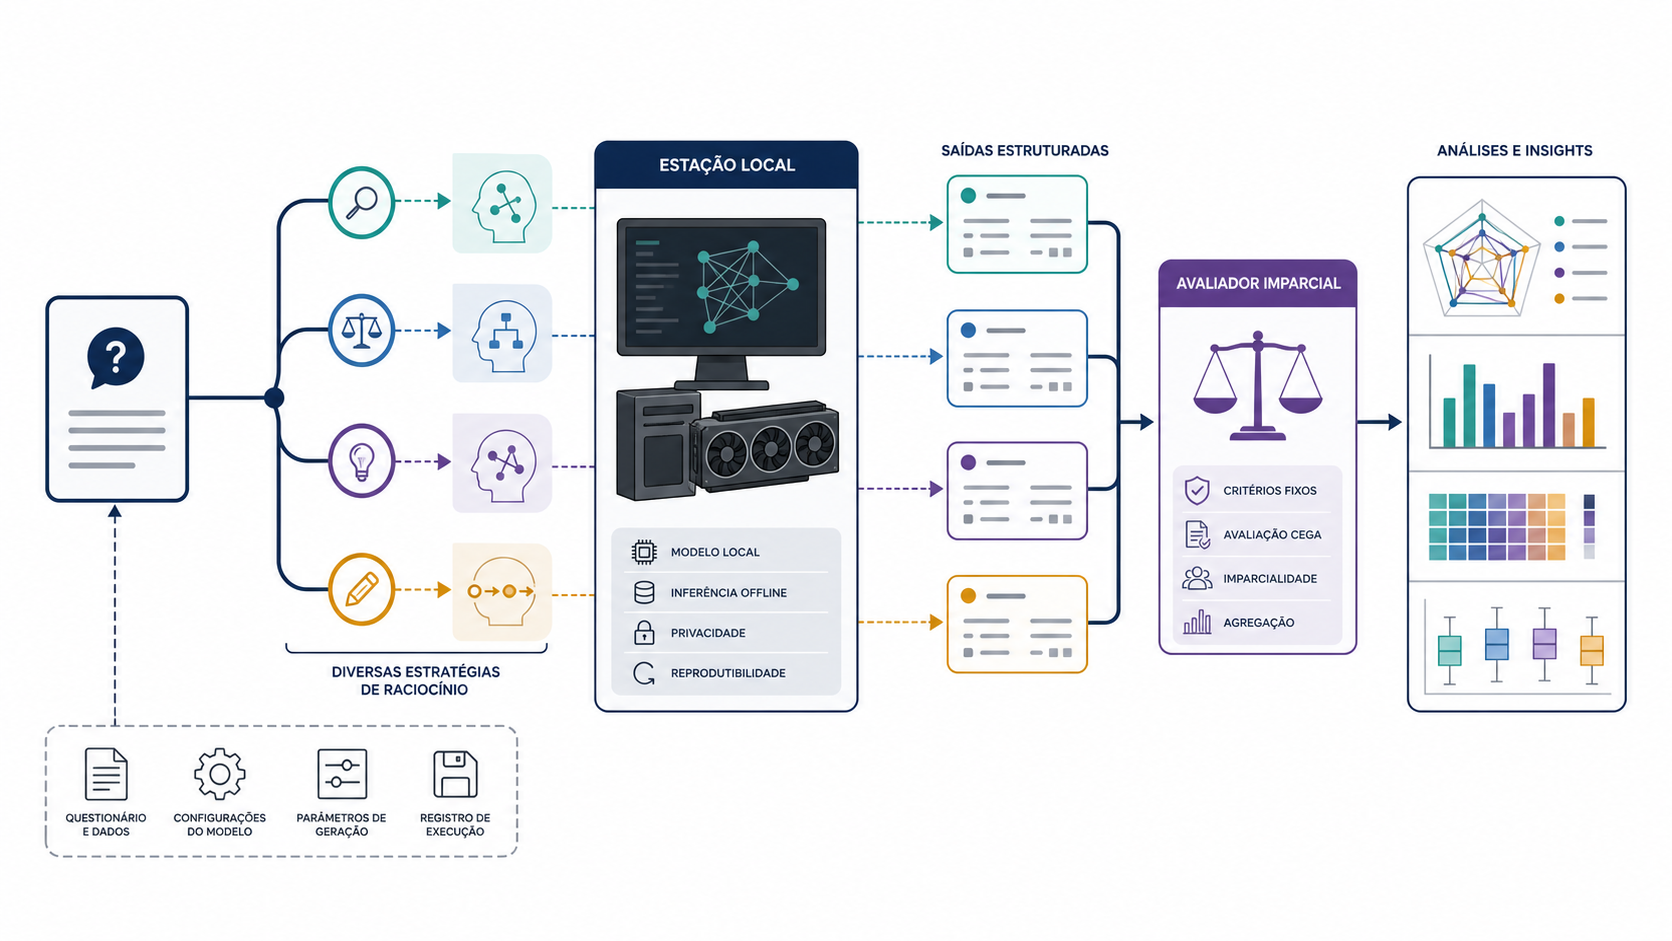
\includegraphics[width=0.98\textwidth]{figuras/fluxo_experimental_ilustrado.png}
\caption{Ilustra\c{c}\~ao conceitual do fluxo reprodut\'ivel: uma pergunta \'{e} processada por estrat\'egias de racioc\'inio, gera sa\'idas estruturadas, passa por avalia\c{c}\~ao independente e produz m\'etricas. A figura \'{e} apenas esquem\'atica e n\~ao representa resultados quantitativos.}
\label{fig:fluxo-ilustrado}
\end{figure}

Esse fluxo separa geração e avaliação. O modelo alvo produz respostas, mas não decide sua própria correção final. A etapa de LLM-juiz atua posteriormente, recebendo gabarito e todas as respostas geradas para a mesma pergunta quando a avaliação determinística não é suficiente ou quando o dataset é semântico, como TruthfulQA. Cada julgamento continua comparativo, mas é repetido com ordem inversa para possibilitar a auditoria de viés posicional.

\subsection{Persistência e Auditoria}

Cada experimento cria uma pasta de rodada com timestamp. Nela são gravados JSON consolidado, JSONL parcial, log textual, manifesto de execução e resumo de recursos. O manifesto registra seed, IDs amostrados, hash dos prompts, versões de bibliotecas, versão do Ollama, plataforma e identificação do modelo quando disponível.

Cada registro contém identificador da instância, índice original, seed, modelo, dataset, abordagem, pergunta, gabarito, resposta gerada, rastros, seleção de \texttt{gflow}, status, duração, número de chamadas, tokens de entrada e saída, duração reportada pelo backend e taxa de tokens por segundo. Um monitor registra ainda picos de RAM do processo, memória do sistema e VRAM quando \texttt{nvidia-smi} está disponível.

\subsection{Amostra Congelada e Bra\c{c}o de Modelo Externo}

Para garantir que a compara\c{c}\~ao entre modelos use exatamente as mesmas inst\^ancias, a rodada congela a amostra antes da infer\^encia externa. As perguntas s\~ao separadas das refer\^encias: o Nemotron recebe somente o arquivo de perguntas, enquanto o arquivo de gabaritos \'{e} utilizado depois, no registro e na avalia\c{c}\~ao. O esquema da Figura~\ref{fig:amostra-congelada} tamb\'em explicita que a compara\c{c}\~ao \texttt{base}--\texttt{cot}--\texttt{for}--\texttt{gflow} ocorre dentro do Gemma, ao passo que o Nemotron constitui um bra\c{c}o de modelo separado.

\begin{figure}[ht]
\centering
\resizebox{\textwidth}{!}{%
\begin{tikzpicture}[
  caixa/.style={draw, rounded corners=3pt, align=center, minimum width=2.65cm, minimum height=1.05cm, font=\small},
  seta/.style={-{Latex[length=2.1mm]}, thick},
  dado/.style={caixa, fill=teal!10, draw=teal!70!black},
  modelo/.style={caixa, fill=blue!8, draw=blue!65!black},
  avaliacao/.style={caixa, fill=purple!10, draw=purple!70!black},
  saida/.style={caixa, fill=orange!12, draw=orange!80!black}
]
\node[dado] (perguntas) {Perguntas\\congeladas};
\node[dado, below=1.0cm of perguntas] (referencias) {Refer\^encias\\e gabaritos};
\node[modelo, right=2.0cm of perguntas] (gemma) {Gemma 4 local\\\texttt{base}, \texttt{cot}, \texttt{for}, \texttt{gflow}};
\node[modelo, right=2.0cm of referencias] (nemotron) {Nemotron Diffusion\\\texttt{base}, carregado uma vez};
\node[saida, right=2.0cm of gemma, yshift=-0.95cm] (respostas) {Respostas e\\telemetria};
\node[avaliacao, right=2.0cm of respostas] (juiz) {Matching determin\'istico\\+ LLM-as-a-Judge};
\node[saida, right=2.0cm of juiz] (metricas) {M\'etricas, testes\\e gr\'aficos};
\draw[seta] (perguntas) -- (gemma);
\draw[seta] (perguntas) |- (nemotron);
\draw[seta] (gemma) -- (respostas);
\draw[seta] (nemotron) -| (respostas);
\draw[seta, dashed] (referencias) -| node[pos=0.25, below, font=\scriptsize] {uso somente na avalia\c{c}\~ao} (juiz);
\draw[seta] (respostas) -- (juiz);
\draw[seta] (juiz) -- (metricas);
\end{tikzpicture}%
}
\caption{Esquema do desenho pareado entre estrat\'egias de prompting do Gemma e baseline externo Nemotron. As perguntas s\~ao as mesmas nos dois bra\c{c}os; os gabaritos n\~ao s\~ao apresentados ao gerador.}
\label{fig:amostra-congelada}
\end{figure}

\subsection{Avaliação}

A avaliação combina três camadas. A primeira é a extração da resposta final. A segunda usa métricas determinísticas: alternativa exata no ARC, comparação numérica no GSM8K e equivalência simbólica via SymPy no MATH/AIME. A terceira é o LLM-as-a-Judge externo, usado para equivalência semântica, TruthfulQA e casos não resolvidos de forma objetiva.

O juiz recebe um payload comparativo por pergunta, inicialmente em ordem embaralhada por seed e depois em ordem inversa. O juiz primário configurado para a rodada integral é \texttt{deepseek/deepseek-v4-flash}. Para o Gemma, o conteúdo inclui pergunta, referência, listas corretas/incorretas do TruthfulQA e as respostas das quatro estratégias. Nos datasets objetivos, esse payload só é encaminhado ao juiz quando a extração ou a equivalência determinística não produz veredito conclusivo; em TruthfulQA, o juiz permanece como avaliador principal. O baseline Nemotron é julgado com a mesma referência, porém em grupo de modelo separado; assim, o ranking de prompting não confunde efeito de prompt com diferença de arquitetura. Para \texttt{gflow}, o juiz avalia oficialmente apenas a resposta selecionada; os rastros alimentam exclusivamente \oracle{}. Uma amostra configurável, por padrão 10\%, pode ser enviada a um segundo juiz externo.

O juiz retorna um JSON estruturado com veredito bin\'ario, pontua\c{c}\~ao, resposta extra\'ida, refer\^encia curta, justificativa, confian\c{c}a e, quando aplic\'avel, categorias de erro, m\'etricas espec\'ificas de TruthfulQA e diagn\'ostico \oracle{}. Esses campos s\~ao mantidos nos artefatos de auditoria, enquanto o artigo reporta apenas as m\'etricas agregadas necess\'arias para a an\'alise quantitativa.

A acurácia é calculada separadamente para cada estratégia \(s\) e dataset \(D\), considerando apenas o conjunto \(V_{s,D}\) de instâncias com veredito válido. Uma instância é incluída em \(V_{s,D}\) quando a comparação determinística, a equivalência simbólica ou o LLM-juiz produz uma decisão binária conclusiva. Casos sem veredito válido são preservados nos artefatos de auditoria, mas não são automaticamente convertidos em erro do modelo, pois representam falha ou inconclusão do procedimento de avaliação, não necessariamente da resposta gerada.

\begin{equation}
Acc(s,D)=
\frac{\sum_{i \in V_{s,D}} \mathbb{1}[\text{resposta}_{s,i}\text{ correta}]}
{|V_{s,D}|}
\end{equation}

Em todas as tabelas, o denominador efetivo é reportado como número de respostas avaliadas ou descrito em nota metodológica. Essa decisão corresponde a uma análise por casos completos e evita misturar erro de geração com ausência de decisão avaliativa.

O ganho em relação à linha de base é calculado pela diferença entre a acurácia da estratégia avaliada e a acurácia da abordagem \texttt{base} no mesmo dataset:

\begin{equation}
\Delta(s,D)=Acc(s,D)-Acc(base,D)
\end{equation}

Dessa forma, valores positivos de \(\Delta(s,D)\) indicam melhora em relação à linha de base, enquanto valores negativos indicam desempenho inferior. Como todas as estratégias respondem às mesmas instâncias, a comparação é pareada. O pipeline calcula Win/Tie/Loss, teste exato de McNemar e correção de Holm para comparações múltiplas. Quando há mais de um SLM, todas as chaves preservam o campo \texttt{modelo}.

\subsection{Métricas de Avaliação Robusta}

\textit{Exact Match} exige igualdade após normalização textual. \textit{Answer Match} aceita equivalência adequada ao domínio: letra correta em múltipla escolha, igualdade numérica em GSM8K, equivalência simbólica em MATH/AIME e equivalência semântica julgada externamente em TruthfulQA. A \textit{Symbolic Equivalence} simplifica a diferença entre expressões com SymPy e considera equivalentes aquelas cujo resultado é zero.

Em TruthfulQA, \textit{Truthfulness} mede se a resposta evita afirmações falsas, enquanto \textit{Informativeness} verifica se ela fornece conteúdo útil em vez de apenas recusar ou responder de forma vaga. Para \texttt{gflow}, \oracle{} representa a proporção de instâncias em que pelo menos uma trajetória estava correta, funcionando como limite superior da exploração multi-trajetória.

A incerteza da acurácia e do delta pareado é estimada por intervalo de confiança de 95\% via bootstrap com 5000 reamostragens. Agreement e Cohen's Kappa são calculados entre juiz primário e ordem reversa e, quando disponíveis, entre juiz primário e segundo juiz e entre juiz e avaliação humana. A taxa de divergência entre ordem original e inversa define o \textit{Position Bias Rate}.

Para relacionar qualidade e custo, são calculadas \textit{Accuracy per Second} e \textit{Gain per Extra Call}. A primeira divide a acurácia pelo tempo médio de parede; a segunda divide o ganho sobre a linha de base pelo número adicional de chamadas ao SLM. Como CoT e FoR possuem o mesmo número de chamadas da base, \textit{Gain per Extra Call} é reportado principalmente para \texttt{gflow}.


\subsection{An\'alise de Erros e Efici\^encia}

Al\'em do veredito bin\'ario, o avaliador registra categorias de erro, como c\'alculo, erro conceitual, formato, premissa falsa, resposta incompleta ou aus\^encia de resposta. Essas categorias permanecem nos arquivos JSON/CSV da rodada e apoiam inspe\c{c}\~oes qualitativas, mas n\~ao s\~ao usadas como denominador principal da acur\'acia. No corpo do artigo, elas s\~ao tratadas como evid\^encia auxiliar para interpretar falhas recorrentes das estrat\'egias.

\subsection{Custo Computacional e Lat\^encia}

O protocolo mede duração de parede, duração reportada pelo backend, tokens de entrada e saída, tokens por segundo, chamadas ao SLM e picos de memória. Essas medidas permitem distinguir uma estratégia lenta por geração extensa de outra limitada por fila, carregamento ou recursos de hardware.

O custo esperado varia conforme a estratégia. A linha de base, CoT e FoR usam uma chamada principal ao SLM. A abordagem \texttt{gflow} exige três chamadas, uma para cada trajetória. Portanto, cada pergunta consome seis chamadas locais quando consideradas as quatro estratégias do Gemma em conjunto. O consenso de \texttt{gflow} é determinístico e não adiciona chamada de modelo.

Na execução integral, com quatro datasets e 100 perguntas por dataset, o Gemma consumiu 2400 chamadas locais: uma para \texttt{base}, \texttt{cot} e \texttt{for}, e três para \texttt{gflow}. A inclusão do baseline Nemotron acrescentou 400 inferências, totalizando 2800 chamadas de geração. O custo temporal entre os dois modelos deve ser interpretado com cautela, pois depende do backend, do dispositivo e do orçamento de tokens de cada execução.

O LLM-juiz opera em duas passagens, ordem original e inversa. Quando todas as instâncias são encaminhadas ao juiz, isso corresponderia a 800 chamadas para os grupos do Gemma e a 800 para os grupos do Nemotron. Na configuração adotada, com \texttt{deepseek/deepseek-v4-flash} como juiz primário, o filtro determinístico reteve TruthfulQA e apenas os casos objetivos sem veredito por código; por isso, a rodada final registrou 660 avaliações por LLM-juiz, abaixo do limite teórico. A avaliação humana permaneceu como etapa preparada pelo pipeline, mas não foi preenchida nesta rodada.

Na continuação sem TruthfulQA, quando executada, a geração mantém o custo local das quatro estratégias sobre GSM8K, ARC-Challenge e Hendrycks MATH/AIME, mas a avaliação externa tende a ser substancialmente menor: apenas respostas objetivas que falham na extração, normalização ou equivalência simbólica são encaminhadas ao juiz. Essa separação torna a ampliação da amostra mais barata e metodologicamente mais robusta, pois a maior parte dos vereditos passa a depender de comparação determinística auditável.

Os gráficos incluem Answer Match, Exact Match, equivalência simbólica, Truthfulness, Informativeness, \oracle{}, Win/Tie/Loss, Position Bias Rate, Accuracy per Second, Gain per Extra Call e custo temporal versus acurácia.


\subsection{Implementa\c{c}\~ao e Artefatos Reprodut\'iveis}

A implementa\c{c}\~ao foi organizada em m\'odulos independentes para permitir repetir gera\c{c}\~ao, avalia\c{c}\~ao, consolida\c{c}\~ao e visualiza\c{c}\~ao sem misturar rodadas. Os detalhes script a script, exemplos completos de JSON e estrutura de pastas s\~ao mantidos no reposit\'orio; aqui, resume-se apenas a fun\c{c}\~ao de cada etapa do protocolo.

\begin{table}[ht]
\centering
\small
\caption{Etapas implementadas e artefatos produzidos.}
\label{tab:artefatos_reprodutiveis}
\begin{tabular}{|p{2.8cm}|p{5.0cm}|p{5.0cm}|}
\hline
\textbf{Etapa} & \textbf{Fun\c{c}\~ao} & \textbf{Artefatos principais} \\
\hline
Gera\c{c}\~ao & Amostrar perguntas, executar Gemma nas quatro estrat\'egias e congelar a amostra. & JSON/JSONL de respostas, manifesto, logs, perguntas e refer\^encias amostradas. \\
\hline
Baseline externo & Executar o Nemotron apenas na condi\c{c}\~ao \texttt{base}, sobre as mesmas perguntas congeladas. & Respostas do modelo externo e telemetria em diret\'orio separado. \\
\hline
Avalia\c{c}\~ao & Aplicar matching determin\'istico, equival\^encia simb\'olica e LLM-as-a-Judge quando necess\'ario. & Vereditos, auditoria de ordem reversa, resumos CSV e registros comparativos. \\
\hline
Consolida\c{c}\~ao e gr\'aficos & Calcular m\'etricas, testes pareados, bootstrap e figuras finais. & Tabelas anal\'iticas, intervalos de confian\c{c}a, Win/Tie/Loss, \oracle{} e gr\'aficos. \\
\hline
\end{tabular}
\end{table}

Os resultados s\~ao organizados por rodada em \texttt{resultados/rodada\_<timestamp>/}. Cada registro preserva seed, modelo, dataset, abordagem, resposta final, status, telemetria e, quando aplic\'avel, rastros de \texttt{gflow}. Essa persist\^encia permite auditar uma inst\^ancia espec\'ifica e retomar etapas interrompidas sem repetir infer\^encias j\'a conclu\'idas.

\section{Resultados da Rodada Final}

Esta seção reporta a rodada final \texttt{rodada\_20260624\_040601}, concluída entre 24 e 25 de junho de 2026. A amostra contém 100 instâncias por dataset, totalizando 400 perguntas congeladas. O Gemma 4 foi executado nas quatro estratégias, produzindo 1600 respostas oficiais; o Nemotron Diffusion respondeu às mesmas 400 perguntas apenas na condição \texttt{base}. Assim, a análise consolida 2000 respostas. Não houve interrupções no processo de geração das respostas. Entretanto, uma parcela dos registros submetidos à etapa de julgamento não recebeu veredito binário válido; esses casos foram preservados nos artefatos de auditoria e excluídos do denominador de acurácia, conforme o critério definido na Seção de Avaliação.

O processamento final registrou 2000 tentativas de avaliação determinística, 660 chamadas ao LLM-juiz, 5000 iterações de bootstrap e seed \texttt{20260612}. O juiz externo foi acionado apenas quando o matching determinístico ou simbólico não produziu veredito conclusivo, ou quando o dataset exigia avaliação semântica, como em TruthfulQA. Para as estratégias do Gemma, 371 respostas por abordagem receberam veredito válido; para o Nemotron, 398 respostas receberam veredito válido. A Tabela~\ref{tab:resultado-final-agregado} resume o resultado agregado.

\noindent\textit{Nota metodológica.} A auditoria dos artefatos da rodada identificou registros sem veredito válido concentrados em um subconjunto restrito de grupos de perguntas. Esses casos decorreram de inconclusões do avaliador automático, como falhas de resposta do serviço externo ou saídas em formato JSON inválido. Como medida conservadora, tais registros não foram imputados como acertos nem como erros. Em Hendrycks MATH/AIME, também foram observadas saídas longas e respostas sem o marcador \texttt{RESPOSTA\_FINAL}, indicando que parte da dificuldade do dataset está associada ao limite de geração e à extração da resposta final. Esses eventos são tratados como limitação operacional da configuração experimental e retomados nas ameaças à validade.

\begin{table}[ht]
\centering
\scriptsize
\setlength{\tabcolsep}{3pt}
\renewcommand{\arraystretch}{1.15}
\caption{Resultado agregado da rodada final. Os intervalos são IC 95\% por bootstrap.}
\label{tab:resultado-final-agregado}
\begin{tabular}{|p{4.0cm}|c|c|c|c|c|}
\hline
\textbf{Modelo / condição} & \textbf{Avaliadas} & \textbf{Corretas} & \textbf{Acurácia} & \textbf{IC 95\%} & \textbf{Chamadas SLM} \\
\hline
Gemma 4 / \texttt{base} & 371 & 317 & \textbf{85,4\%} & [81,7\%; 89,0\%] & 400 \\
Gemma 4 / \texttt{cot} & 371 & 309 & 83,3\% & [79,3\%; 87,1\%] & 400 \\
Gemma 4 / \texttt{for} & 371 & 308 & 83,0\% & [79,0\%; 86,8\%] & 400 \\
Gemma 4 / \texttt{gflow} & 371 & 306 & 82,5\% & [78,4\%; 86,3\%] & 1200 \\
Nemotron Diffusion / \texttt{base} & 398 & 158 & 39,7\% & [34,7\%; 44,5\%] & 400 \\
\hline
\end{tabular}
\end{table}

O principal resultado é negativo para a hipótese de superioridade geral das estratégias estruturadas: na agregação final, a linha de base direta do Gemma obteve a maior acurácia. O CoT ficou 2,15 pontos percentuais abaixo da base; o FoR, 2,42 pontos abaixo; e o \texttt{gflow}, 2,96 pontos abaixo. Como as estratégias foram aplicadas às mesmas instâncias, a comparação pareada é mais informativa que a diferença agregada bruta. Nessa análise, nenhuma estratégia estruturada apresentou ganho estatisticamente robusto sobre a linha de base após correção de Holm.


\begin{figure}[ht]
\centering
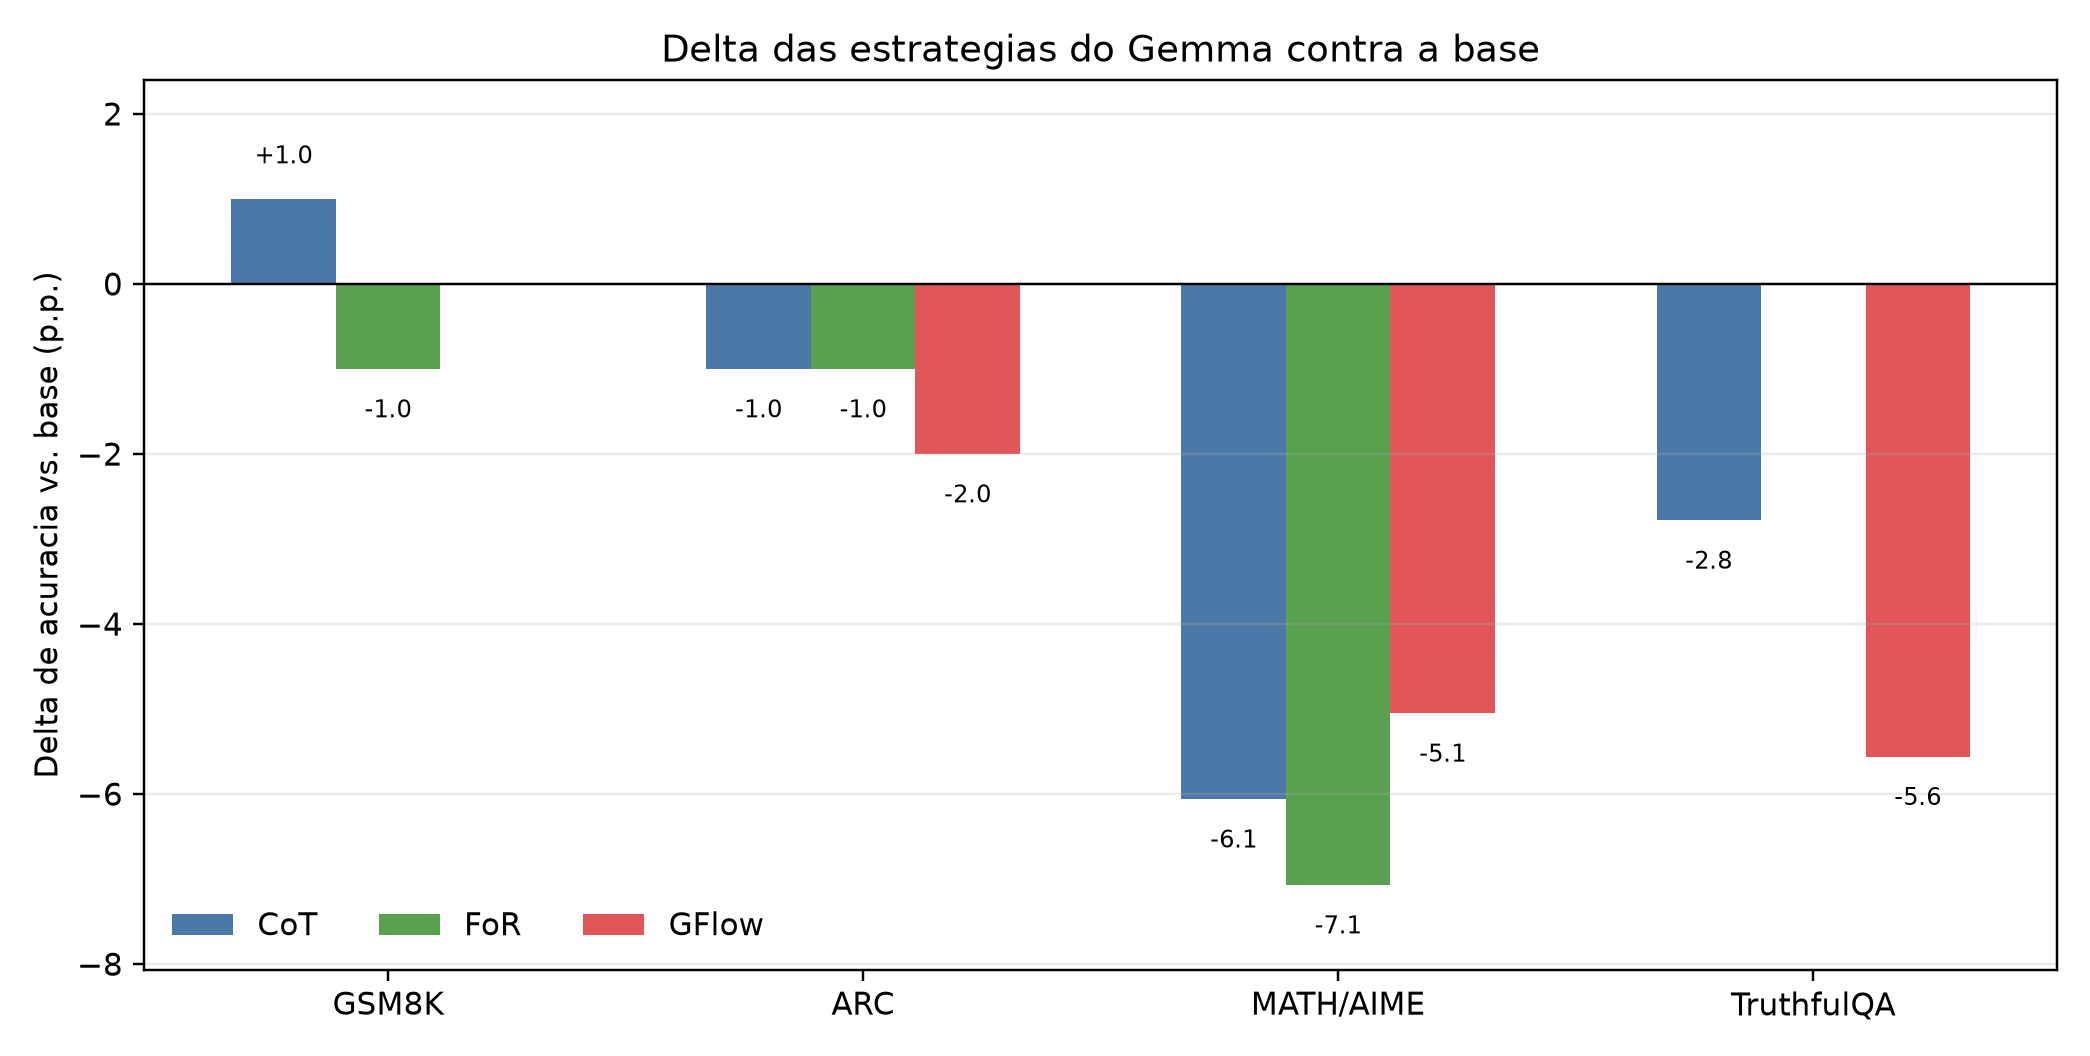
\includegraphics[width=0.92\textwidth]{figuras/delta_vs_base_gemma_limpo.png}
\caption{Delta de acur\'acia das estrat\'egias estruturadas contra a linha de base do Gemma. Valores positivos indicam ganho sobre \texttt{base}; valores negativos indicam perda.}
\label{fig:delta-base-final}
\end{figure}

\subsection{Resultados por Dataset}

A Tabela~\ref{tab:resultado-final-dataset} mostra que o efeito das estratégias varia por domínio. Em ARC-Challenge, o desempenho do Gemma ficou próximo do teto para todas as estratégias, com pequena vantagem da linha de base. Em GSM8K, CoT obteve o único ganho positivo observado contra a base, mas de apenas um ponto percentual. Em Hendrycks MATH/AIME, as três estratégias estruturadas ficaram abaixo da resposta direta. Em TruthfulQA, \texttt{base} e FoR empataram em acurácia, mas FoR obteve a maior Informativeness entre as estratégias do Gemma.

\begin{table}[ht]
\centering
\scriptsize
\setlength{\tabcolsep}{3pt}
\renewcommand{\arraystretch}{1.15}
\caption{Acurácia por dataset na rodada final. Valores em porcentagem.}
\label{tab:resultado-final-dataset}
\begin{tabular}{|p{3.0cm}|c|c|c|c|c|}
\hline
\textbf{Dataset} & \textbf{G-base} & \textbf{G-CoT} & \textbf{G-FoR} & \textbf{G-GFlow} & \textbf{N-base} \\
\hline
ARC-Challenge & \textbf{97,0} & 96,0 & 96,0 & 95,0 & 83,0 \\
GSM8K & 92,0 & \textbf{93,0} & 91,0 & 92,0 & 19,0 \\
Hendrycks MATH/AIME & \textbf{81,8} & 75,8 & 74,7 & 76,8 & 12,1 \\
TruthfulQA & \textbf{65,3} & 62,5 & \textbf{65,3} & 59,7 & 44,4 \\
\hline
\end{tabular}
\par\vspace{0.4em}
\begin{minipage}{0.95\textwidth}
\footnotesize\textit{Nota:} As porcentagens por dataset foram calculadas apenas sobre respostas com veredito válido. Para Gemma, \(n\) válido por abordagem foi ARC=100, GSM8K=100, Hendrycks MATH/AIME=99 e TruthfulQA=72; para Nemotron, \(n=100\), \(100\), \(99\) e \(99\), respectivamente. Casos inconclusivos do avaliador foram mantidos fora do denominador, razão pela qual alguns valores não correspondem exatamente a múltiplos de 1 ponto percentual.
\end{minipage}
\end{table}

Os testes Win/Tie/Loss reforçam essa leitura. Em ARC-Challenge, as comparações contra a base tiveram 95\% ou mais de empates. Em GSM8K, CoT venceu uma instância adicional e não perdeu nenhuma, mas o teste de McNemar permaneceu inconclusivo. Em Hendrycks MATH/AIME, FoR teve perda pareada de 7,07 pontos percentuais contra a base; ainda assim, após correção de Holm, a diferença não atingiu evidência estatística robusta. Em TruthfulQA, FoR empatou com a base, enquanto CoT e \texttt{gflow} ficaram abaixo.

\begin{figure}[ht]
\centering
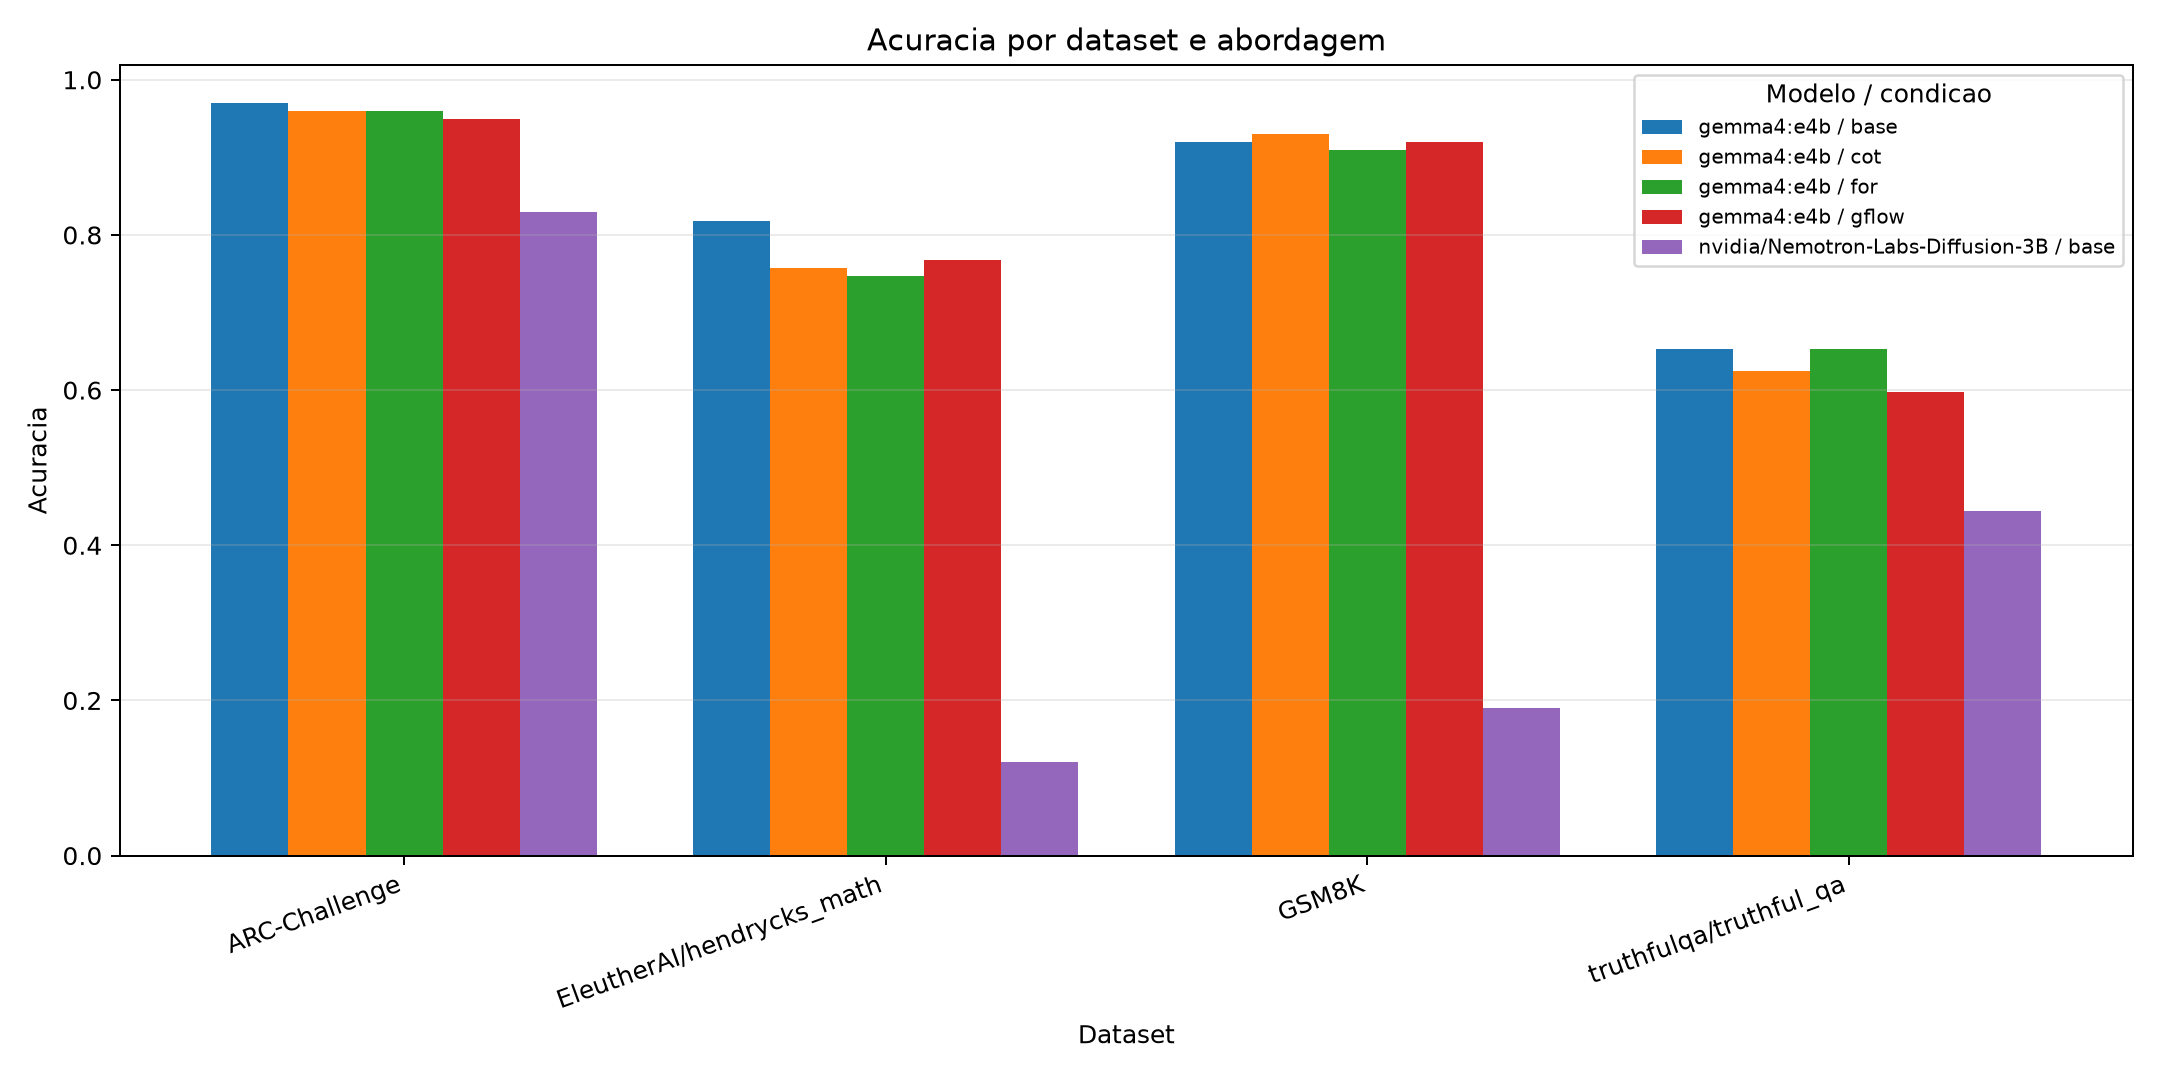
\includegraphics[width=0.98\textwidth]{figuras/acuracia_final_por_dataset_abordagem.png}
\caption{Acurácia por dataset e condição. A figura evidencia que a comparação agregada esconde comportamentos distintos por domínio.}
\label{fig:acuracia-final-dataset}
\end{figure}

\subsection{Multi-trajetória e \oracle{}}

A estratégia \texttt{gflow} apresentou o maior custo computacional relativo entre as abordagens do Gemma, pois exige três chamadas ao SLM por instância. Sua acurácia oficial, contudo, foi inferior à linha de base agregada. O diagnóstico \oracle{} mostra que ao menos uma das três trajetórias frequentemente continha uma resposta correta, mas o consenso determinístico nem sempre selecionou essa alternativa. Portanto, os resultados sugerem que a limitação principal está no mecanismo de seleção das trajetórias, e não apenas na capacidade de gerar candidatos diversos.

\begin{table}[ht]
\centering
\scriptsize
\setlength{\tabcolsep}{4pt}
\renewcommand{\arraystretch}{1.15}
\caption{Acurácia oficial de \texttt{gflow} e teto diagnóstico \oracle{}.}
\label{tab:oracle-final}
\begin{tabular}{|p{3.6cm}|c|c|c|}
\hline
\textbf{Dataset} & \textbf{Acurácia oficial} & \textbf{\oracle{}} & \textbf{Diferença} \\
\hline
ARC-Challenge & 95,0\% & 99,0\% & +4,0 p.p. \\
GSM8K & 92,0\% & 93,0\% & +1,0 p.p. \\
Hendrycks MATH/AIME & 76,8\% & 79,8\% & +3,0 p.p. \\
TruthfulQA & 59,7\% & 66,7\% & +6,9 p.p. \\
Agregado & 82,5\% & 86,0\% & +3,5 p.p. \\
\hline
\end{tabular}
\end{table}

Essa diferença é metodologicamente relevante. Se \texttt{gflow} fosse avaliado pelo melhor dos três caminhos, seu desempenho se aproximaria ou superaria a base agregada. Porém, esse cenário seria oracular, pois exigiria saber qual trajetória está correta. Na condição operacional real, a seleção por consenso não apresentou evidência empírica suficiente para compensar o aumento de custo sob a configuração avaliada.


\begin{figure}[ht]
\centering
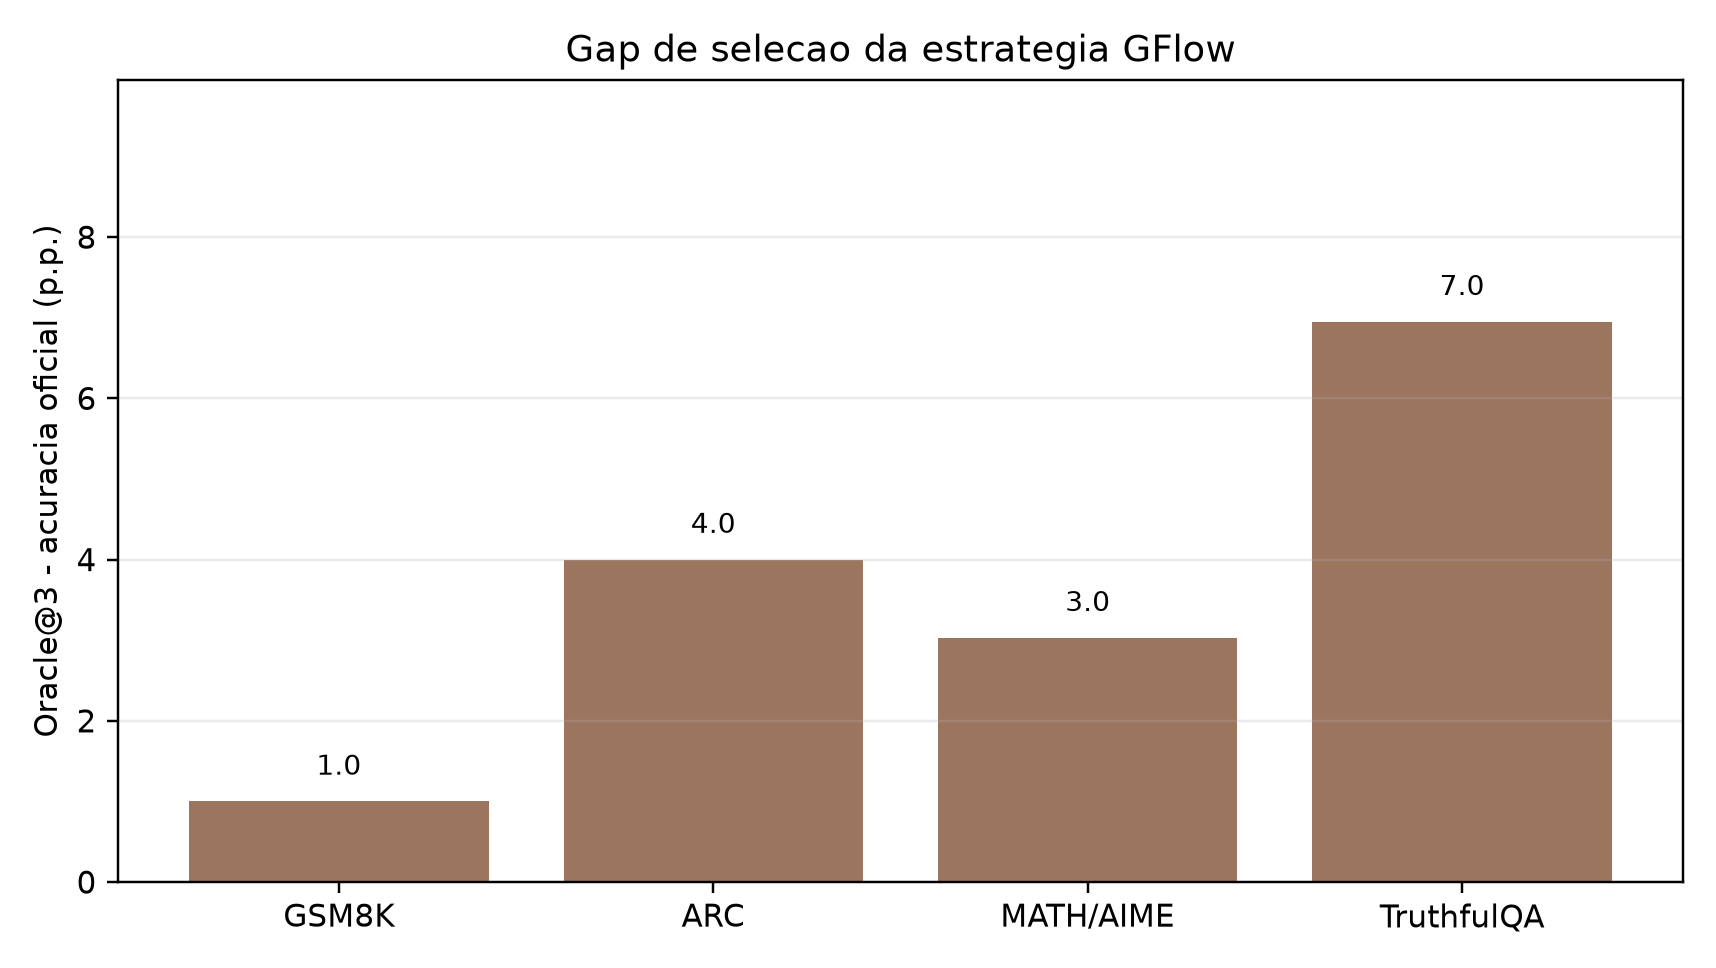
\includegraphics[width=0.82\textwidth]{figuras/oracle_gap_gflow.png}
\caption{Gap entre \oracle{} e a acur\'acia oficial da estrat\'egia \texttt{gflow}. O gr\'afico evidencia o potencial perdido na etapa de sele\c{c}\~ao das trajet\'orias.}
\label{fig:oracle-final}
\end{figure}

\subsection{Comparação com Nemotron Diffusion}

O Nemotron Diffusion foi incluído como baseline externo de modelo, não como uma quinta estratégia de prompting do Gemma. A comparação usa as mesmas perguntas congeladas, mas deve ser lida como comparação de correção sob condições de execução distintas. Em todos os datasets, o baseline Gemma superou o baseline Nemotron.

\begin{table}[ht]
\centering
\scriptsize
\setlength{\tabcolsep}{4pt}
\renewcommand{\arraystretch}{1.15}
\caption{Comparação pareada entre Nemotron \texttt{base} e Gemma \texttt{base}.}
\label{tab:nemotron-final}
\begin{tabular}{|p{3.2cm}|c|c|c|c|c|}
\hline
\textbf{Dataset} & \textbf{Gemma base} & \textbf{Nemotron base} & \textbf{\(n\) pareado} & \textbf{\(\Delta\) N--G} & \textbf{\(p\) Holm} \\
\hline
ARC-Challenge & 97,0\% & 83,0\% & 100 & -14,0 p.p. & \(0{,}001038\) \\
GSM8K & 92,0\% & 19,0\% & 100 & -73,0 p.p. & \(<0{,}000001\) \\
Hendrycks MATH/AIME & 81,8\% & 12,1\% & 98 & -69,4 p.p. & \(<0{,}000001\) \\
TruthfulQA & 65,3\% & 44,4\% & 72 & -23,6 p.p. & \(0{,}001514\) \\
\hline
\end{tabular}
\vspace{2pt}

\footnotesize\textit{Nota:} As colunas de acurácia usam os vereditos válidos marginais de cada modelo. Já \(\Delta\) N--G e \(p\) Holm são calculados somente nas instâncias pareadas em que Gemma e Nemotron receberam veredito válido; por isso, o delta pode não coincidir exatamente com a subtração direta das duas porcentagens marginais.
\end{table}

O resultado mais distante ocorreu em GSM8K e Hendrycks MATH/AIME, sugerindo fragilidade do Nemotron nesta configuração para tarefas quantitativas e simbólicas. Em TruthfulQA, a diferença foi menor, mas ainda desfavorável. Como o Nemotron gerou respostas muito mais curtas e foi executado por backend distinto, os números de duração e throughput são mantidos como telemetria, mas não sustentam uma comparação de eficiência entre arquiteturas.

\subsection{Confiabilidade do Juiz}

A auditoria posicional comparou julgamentos em ordem original e ordem inversa. No agregado, foram 530 pares comparáveis, com 96,42\% de concordância, Cohen's Kappa de 0,928 e Position Bias Rate de 3,58\%. A maior taxa por célula do Gemma apareceu em TruthfulQA, chegando a 7,14\% na linha de base. Esses valores sugerem estabilidade razoável do juiz externo, mas não eliminam a necessidade de revisão humana em casos semânticos.

\begin{table}[ht]
\centering
\small
\caption{Auditoria global do LLM-juiz por ordem reversa.}
\label{tab:auditoria-juiz-final}
\begin{tabular}{|l|c|}
\hline
\textbf{Métrica} & \textbf{Valor} \\
\hline
Pares comparáveis & 530 \\
Agreement & 96,42\% \\
Cohen's Kappa & 0,928 \\
Position Bias Rate & 3,58\% \\
Avaliações humanas preenchidas & 0 \\
\hline
\end{tabular}
\end{table}

\subsection{Eficiência}

Entre as estratégias do Gemma, a linha de base apresentou a melhor acurácia agregada por segundo (0,003515), praticamente empatada com CoT (0,003505). FoR e \texttt{gflow} ficaram abaixo, especialmente porque aumentam o comprimento das respostas e, no caso de \texttt{gflow}, triplicam as chamadas por pergunta. Assim, sob a configuração testada, a estratégia direta é o melhor ponto de equilíbrio entre qualidade e custo. CoT pode ser mantido como alternativa quando a tarefa é aritmética, mas a evidência observada é pequena. FoR e \texttt{gflow} exigem melhorias no prompt, na seleção ou no uso seletivo por tipo de problema antes de serem adotados como padrão.


Como s\'intese, a estrat\'egia \texttt{gflow} apresentou o maior custo computacional relativo, por exigir tr\^es chamadas ao SLM por inst\^ancia. Sob a configura\c{c}\~ao avaliada, esse custo adicional n\~ao apresentou evid\^encia emp\'irica suficiente para compensar a acur\'acia agregada inferior \`a linha de base. As figuras de efici\^encia completas permanecem dispon\'iveis no reposit\'orio como artefatos de an\'alise.

\FloatBarrier
\section{Ameaças à Validade}

A primeira ameaça à validade está na avaliação. Mesmo com referência, um LLM-juiz pode cometer erros ou favorecer posições. O estudo mitiga esse risco com avaliação determinística sempre que possível, ordem reversa e cálculo de Agreement, Cohen's Kappa e Position Bias Rate. Ainda assim, a avaliação humana cega não foi preenchida nesta rodada, de modo que a validade semântica de TruthfulQA permanece dependente do juiz externo e das referências disponíveis.

A segunda ameaça está na presença de registros sem veredito válido. Embora a rodada não tenha apresentado interrupções no processo de geração, parte das respostas submetidas à etapa automática de julgamento não produziu decisão binária conclusiva, sobretudo em TruthfulQA. A auditoria identificou 118 linhas sem veredito em 31 grupos de perguntas, associadas principalmente a indisponibilidade intermitente do serviço externo de avaliação e a respostas do juiz em JSON inválido ou malformado. Esses registros foram mantidos nos artefatos de auditoria, mas removidos do denominador de acurácia. A decisão evita penalizar o modelo por uma inconclusão do avaliador; por outro lado, reduz o tamanho efetivo da amostra e pode introduzir viés caso os registros sem veredito não sejam aleatórios.

A terceira ameaça está na extração da resposta final. Embora o marcador \texttt{RESPOSTA\_FINAL} reduza ambiguidade, o modelo pode descumprir o formato solicitado, incluir texto adicional ou atingir o limite de geração antes de emitir a resposta. Esse comportamento apareceu com mais força em Hendrycks MATH/AIME: 52 registros atingiram \texttt{total\_tokens=4096}, 34 ficaram com \texttt{resposta\_gerada} vazia e 72 não continham o marcador esperado. Por isso, o avaliador também tenta reconhecer variações como \texttt{Final answer} e usa a última linha como fallback. Mesmo assim, erros de parsing podem afetar especialmente respostas matemáticas longas ou com notação complexa.

A quarta ameaça está na generalização dos resultados. A rodada final usa 100 perguntas por dataset e um único SLM local como alvo principal. Essa amostra é suficiente para uma comparação pareada inicial, mas ainda limitada diante da diversidade total de problemas, prompts, seeds e versões de modelos. A amostragem estratificada e os intervalos de confiança por bootstrap reduzem, mas não eliminam, essa limitação.

A quinta ameaça é a contaminação de benchmark. Como GSM8K, ARC-Challenge, MATH e TruthfulQA são datasets públicos, os modelos podem ter visto itens semelhantes durante treinamento. Ainda assim, a comparação relativa entre estratégias permanece útil, pois todas respondem às mesmas instâncias sob o mesmo modelo.

Uma ameaça adicional à comparação entre modelos é a assimetria de infraestrutura e backend. O Gemma foi executado localmente via Ollama, enquanto o Nemotron foi executado por PyTorch/Transformers. A amostra comum torna a comparação de correção informativa, mas latência, throughput, consumo de recursos e comprimento de saída não devem ser tratados como comparação direta de eficiência arquitetural.

\section{Considerações Finais}

Este trabalho consolidou e executou um protocolo reprodutível para comparar estratégias de prompting no Gemma 4 e acrescentou um baseline externo com Nemotron Diffusion sobre a mesma amostra congelada. A separação entre perguntas e referências, a persistência dos manifestos, o matching determinístico, a equivalência simbólica e a auditoria do LLM-juiz tornam o fluxo rastreável e permitem repetir geração, avaliação ou análise sem misturar rodadas.

Em relação à QP1, os resultados desta rodada não sustentam ganho agregado das estratégias estruturadas sobre a resposta direta. A linha de base obteve a maior acurácia global entre as condições do Gemma, enquanto CoT apresentou apenas um ganho local em GSM8K. Assim, a evidência sugere que estratégias de raciocínio podem ter efeito dependente do domínio, mas não produziram melhoria geral sob a configuração testada. Em relação à QP2, a estratégia multi-trajetória não apresentou evidência empírica suficiente para compensar o aumento de chamadas na forma atual: o \oracle{} mostra potencial latente, mas o consenso oficial não selecionou esse potencial de modo confiável. Em relação à QP3, o efeito varia por dataset: CoT teve pequeno ganho em GSM8K, FoR empatou com a base em TruthfulQA, e as estratégias estruturadas perderam em Hendrycks MATH/AIME. Em relação à QP4, a padronização da resposta final e a combinação de avaliação determinística com LLM-juiz tornaram a análise auditável, embora a ausência de avaliação humana ainda limite a força das conclusões semânticas.

Como resultado prático, a configuração mais defensável para o Gemma 4 nesta rodada é usar \texttt{base} como padrão geral e reservar CoT para tarefas aritméticas quando o custo de uma resposta mais longa for aceitável. FoR e \texttt{gflow} permanecem promissores como estruturas de pesquisa, mas precisam de seleção mais forte, acionamento seletivo por domínio ou julgamento interno calibrado antes de serem adotados como estratégia padrão. O Nemotron Diffusion, nesta configuração, ficou substancialmente abaixo do Gemma em correção e deve ser tratado apenas como baseline externo exploratório.

\begin{thebibliography}{99}

\bibitem{wei2022}
Wei, J., Wang, X., Schuurmans, D., Bosma, M., Ichter, B., Xia, F., Chi, E., Le, Q. V. and Zhou, D. (2022).
Chain-of-thought prompting elicits reasoning in large language models.
In \textit{Advances in Neural Information Processing Systems}, volume 35.

\bibitem{zhou2023}
Zhou, D., Schärli, N., Hou, L., Wei, J., Scales, N., Wang, X., Schuurmans, D., Cui, C., Bousquet, O., Le, Q. and Chi, E. (2023).
Least-to-most prompting enables complex reasoning in large language models.
In \textit{International Conference on Learning Representations}.


\bibitem{kojima2022}
Kojima, T., Gu, S. S., Reid, M., Matsuo, Y. and Iwasawa, Y. (2022).
Large language models are zero-shot reasoners.
In \textit{Advances in Neural Information Processing Systems}, volume 35.

\bibitem{wang2022selfconsistency}
Wang, X., Wei, J., Schuurmans, D., Le, Q., Chi, E., Narang, S., Chowdhery, A. and Zhou, D. (2022).
Self-consistency improves chain of thought reasoning in language models.
In \textit{International Conference on Learning Representations}.

\bibitem{wang2023plansolve}
Wang, L., Xu, W., Lan, Y., Hu, Z., Lan, Y., Lee, R. K.-W. and Lim, E.-P. (2023).
Plan-and-solve prompting: Improving zero-shot chain-of-thought reasoning by large language models.
In \textit{Proceedings of the 61st Annual Meeting of the Association for Computational Linguistics}, pages 2609--2634.

\bibitem{yao2023tot}
Yao, S., Yu, D., Zhao, J., Shafran, I., Griffiths, T. L., Cao, Y. and Narasimhan, K. (2023).
Tree of thoughts: Deliberate problem solving with large language models.
In \textit{Advances in Neural Information Processing Systems}, volume 36.

\bibitem{mukherjee2023}
Mukherjee, S., Mitra, A., Jawahar, G., Agarwal, S., Palangi, H. and Awadallah, A. (2023).
Orca: Progressive learning from complex explanation traces of GPT-4.
\textit{arXiv preprint arXiv:2306.02707}.

\bibitem{ranaldi2024}
Ranaldi, L. and Freitas, A. (2024).
Aligning large and small language models via chain-of-thought reasoning.
In \textit{Proceedings of the 18th Conference of the European Chapter of the Association for Computational Linguistics}, pages 1812--1827.

\bibitem{thinkslm2025}
Srivastava, G., Cao, S. and Wang, X. (2025).
ThinkSLM: Towards reasoning in small language models.
In \textit{Proceedings of the 2025 Conference on Empirical Methods in Natural Language Processing}, pages 32612--32662.

\bibitem{slmbench2025}
Pham, N. T., Kieu, T., Nguyen, D.-M., Xuan, S. H., Duong-Trung, N. and Le-Phuoc, D. (2025).
SLM-Bench: A comprehensive benchmark of small language models on environmental impacts--Extended version.
\textit{arXiv preprint arXiv:2508.15478}.

\bibitem{cobbe2021}
Cobbe, K., Kosaraju, V., Bavarian, M., Chen, M., Jun, H., Kaiser, L., Plappert, M., Tworek, J., Hilton, J., Nakano, R., Hesse, C. and Schulman, J. (2021).
Training verifiers to solve math word problems.
\textit{arXiv preprint arXiv:2110.14168}.

\bibitem{clark2018}
Clark, P., Cowhey, I., Etzioni, O., Khot, T., Sabharwal, A., Schoenick, C. and Tafjord, O. (2018).
Think you have solved question answering? Try ARC, the AI2 Reasoning Challenge.
\textit{arXiv preprint arXiv:1803.05457}.

\bibitem{hendrycks2021}
Hendrycks, D., Burns, C., Kadavath, S., Arora, A., Basart, S., Tang, E., Song, D. and Steinhardt, J. (2021).
Measuring mathematical problem solving with the MATH dataset.
\textit{NeurIPS Datasets and Benchmarks}.

\bibitem{lin2022}
Lin, S., Hilton, J. and Evans, O. (2022).
TruthfulQA: Measuring how models mimic human falsehoods.
In \textit{Proceedings of the 60th Annual Meeting of the Association for Computational Linguistics}.

\bibitem{zheng2023}
Zheng, L., Chiang, W.-L., Sheng, Y., Zhuang, S., Wu, Z., Zhuang, Y., Lin, Z., Li, Z., Li, D., Xing, E., Zhang, H., Gonzalez, J. and Stoica, I. (2023).
Judging LLM-as-a-judge with MT-Bench and Chatbot Arena.
In \textit{Advances in Neural Information Processing Systems}, volume 36.

\bibitem{zhu2023}
Zhu, L. et al. (2023).
JudgeLM: Fine-tuned large language models are scalable judges.
\textit{arXiv preprint arXiv:2310.17631}.


\bibitem{shi2024position}
Shi, L., Ma, C., Liang, W., Ma, W. and Vosoughi, S. (2024).
Judging the judges: A systematic study of position bias in LLM-as-a-Judge.
\textit{arXiv preprint arXiv:2406.07791}.

\bibitem{bengio2021}
Bengio, E., Jain, M., Korablyov, M., Precup, D. and Bengio, Y. (2021).
Flow network based generative models for non-iterative diverse candidate generation.
In \textit{Advances in Neural Information Processing Systems}.

\end{thebibliography}

\end{document}
